\documentclass[landscape,12pt,openany]{book}

\usepackage{multicol}
\usepackage{graphicx}
\graphicspath{{./images/}}
\usepackage[margin=.5in, paperwidth=9in, paperheight=7in]{geometry}
\usepackage{titlesec}
\usepackage{xfrac}
\usepackage{framed}
\usepackage{gensymb}
\usepackage[abs]{overpic}
\setlength\unitlength{1in}
\usepackage{color}

\usepackage{cookbook}  % custom style

\titlespacing*{\chapter}{0em}{-3em}{1em}
\titleformat{\chapter}{\normalfont\huge\bfseries}{\chaptertitlename\
\thechapter:}{20pt}{\Huge}
\renewcommand{\thesection}{}  % don't show the section numbers
\titleformat{\section}[block]{\titlerule\scshape\large\filcenter\vspace{2pt}}{}{0em}{}[\titlerule]
\titleformat{\subsection}[block]{\scshape\large\filcenter}{}{0em}{}[\titlerule]
\setlength{\parindent}{1em}
\setlength{\columnseprule}{0.4pt}
\pagestyle{plain}
\raggedbottom
\usepackage[utf8]{inputenc}
\usepackage[T1]{fontenc}

\begin{document}

\rmfamily

\begin{titlepage}
    \newgeometry{margin=0in,hmargin=-12pt}
    \begin{overpic}[height=\paperheight,tics=1]{cover.jpg}
        \put(6,6){\Huge\bf\color{white} Cookbook 2013}
        \put(6.85,5.5){\Large\bf\color{white} Chase Seibert}
    \end{overpic}
    \restoregeometry
\end{titlepage}

\columnsep=2em
\setlength{\columnseprule}{0pt}.

\setcounter{page}{0}
\cleardoublepage
\setcounter{tocdepth}{1}
\tableofcontents

\chapter{Salads}
\section{Caesar Salad}
\begin{recipe}

Place serving bowls and large mixing bowl in the freezer.

\ingredients{
    \sfrac{1}{2} & loaf rye bread \\
    \sfrac{1}{4} & cup olive oil \\
              5  & garlic cloves \\
}

Simmer smashed garlic cloves in oil for 10 minutes to flavor the oil.

Cut bread into \sfrac{1}{2} inch cubes. Spread on a baking sheet and paint with olive oil mixture.

Bake at 350\degree{} for 10 minutes, and then continue to bake, watching closely, until golden brown.

Place croûtons in an open container and put in the freezer for 10 minutes.

\ingredients{
   1 & block parmesan reggiano \\
}

Grate 1 cup coarse, and \sfrac{1}{2} cup fine.

\ingredients{
    2 & heads romaine hearts \\
}

Cut into \sfrac{3}{4} inch rounds, separate and then chop roughly.

\ingredientsLeft{
    & dressing \\
    & fresh pepper \\
}

When you're ready to serve, remove large mixing bowl from freezer. Combine lettuce, cheese, pepper and two large spoonfuls of dressing.

Add croûtons, and mix again briefly. Turn out into serving bowls from the freezer.

\subsection{Caesar Dressing}

\ingredients{
               1 & large egg \\
               3 & tablespoons lemon juice \\
               1 & teaspoon Worcestershire \\
   1\sfrac{1}{2} & teaspoon anchovy paste \\
               1 &  clove garlic \\
}

Blanch egg in shell for 45 seconds in boiling water. Remove and crack into a small bowl. Whisk with other ingredients.

\ingredients{
    \sfrac{1}{3} & cup olive oil (extra-virgin) \\
}

Slowly whisk oil into the dressing. Season to taste with salt and pepper.

\end{recipe}

\newgeometry{margin=0in}
\begin{figure}[p]
    \centering
    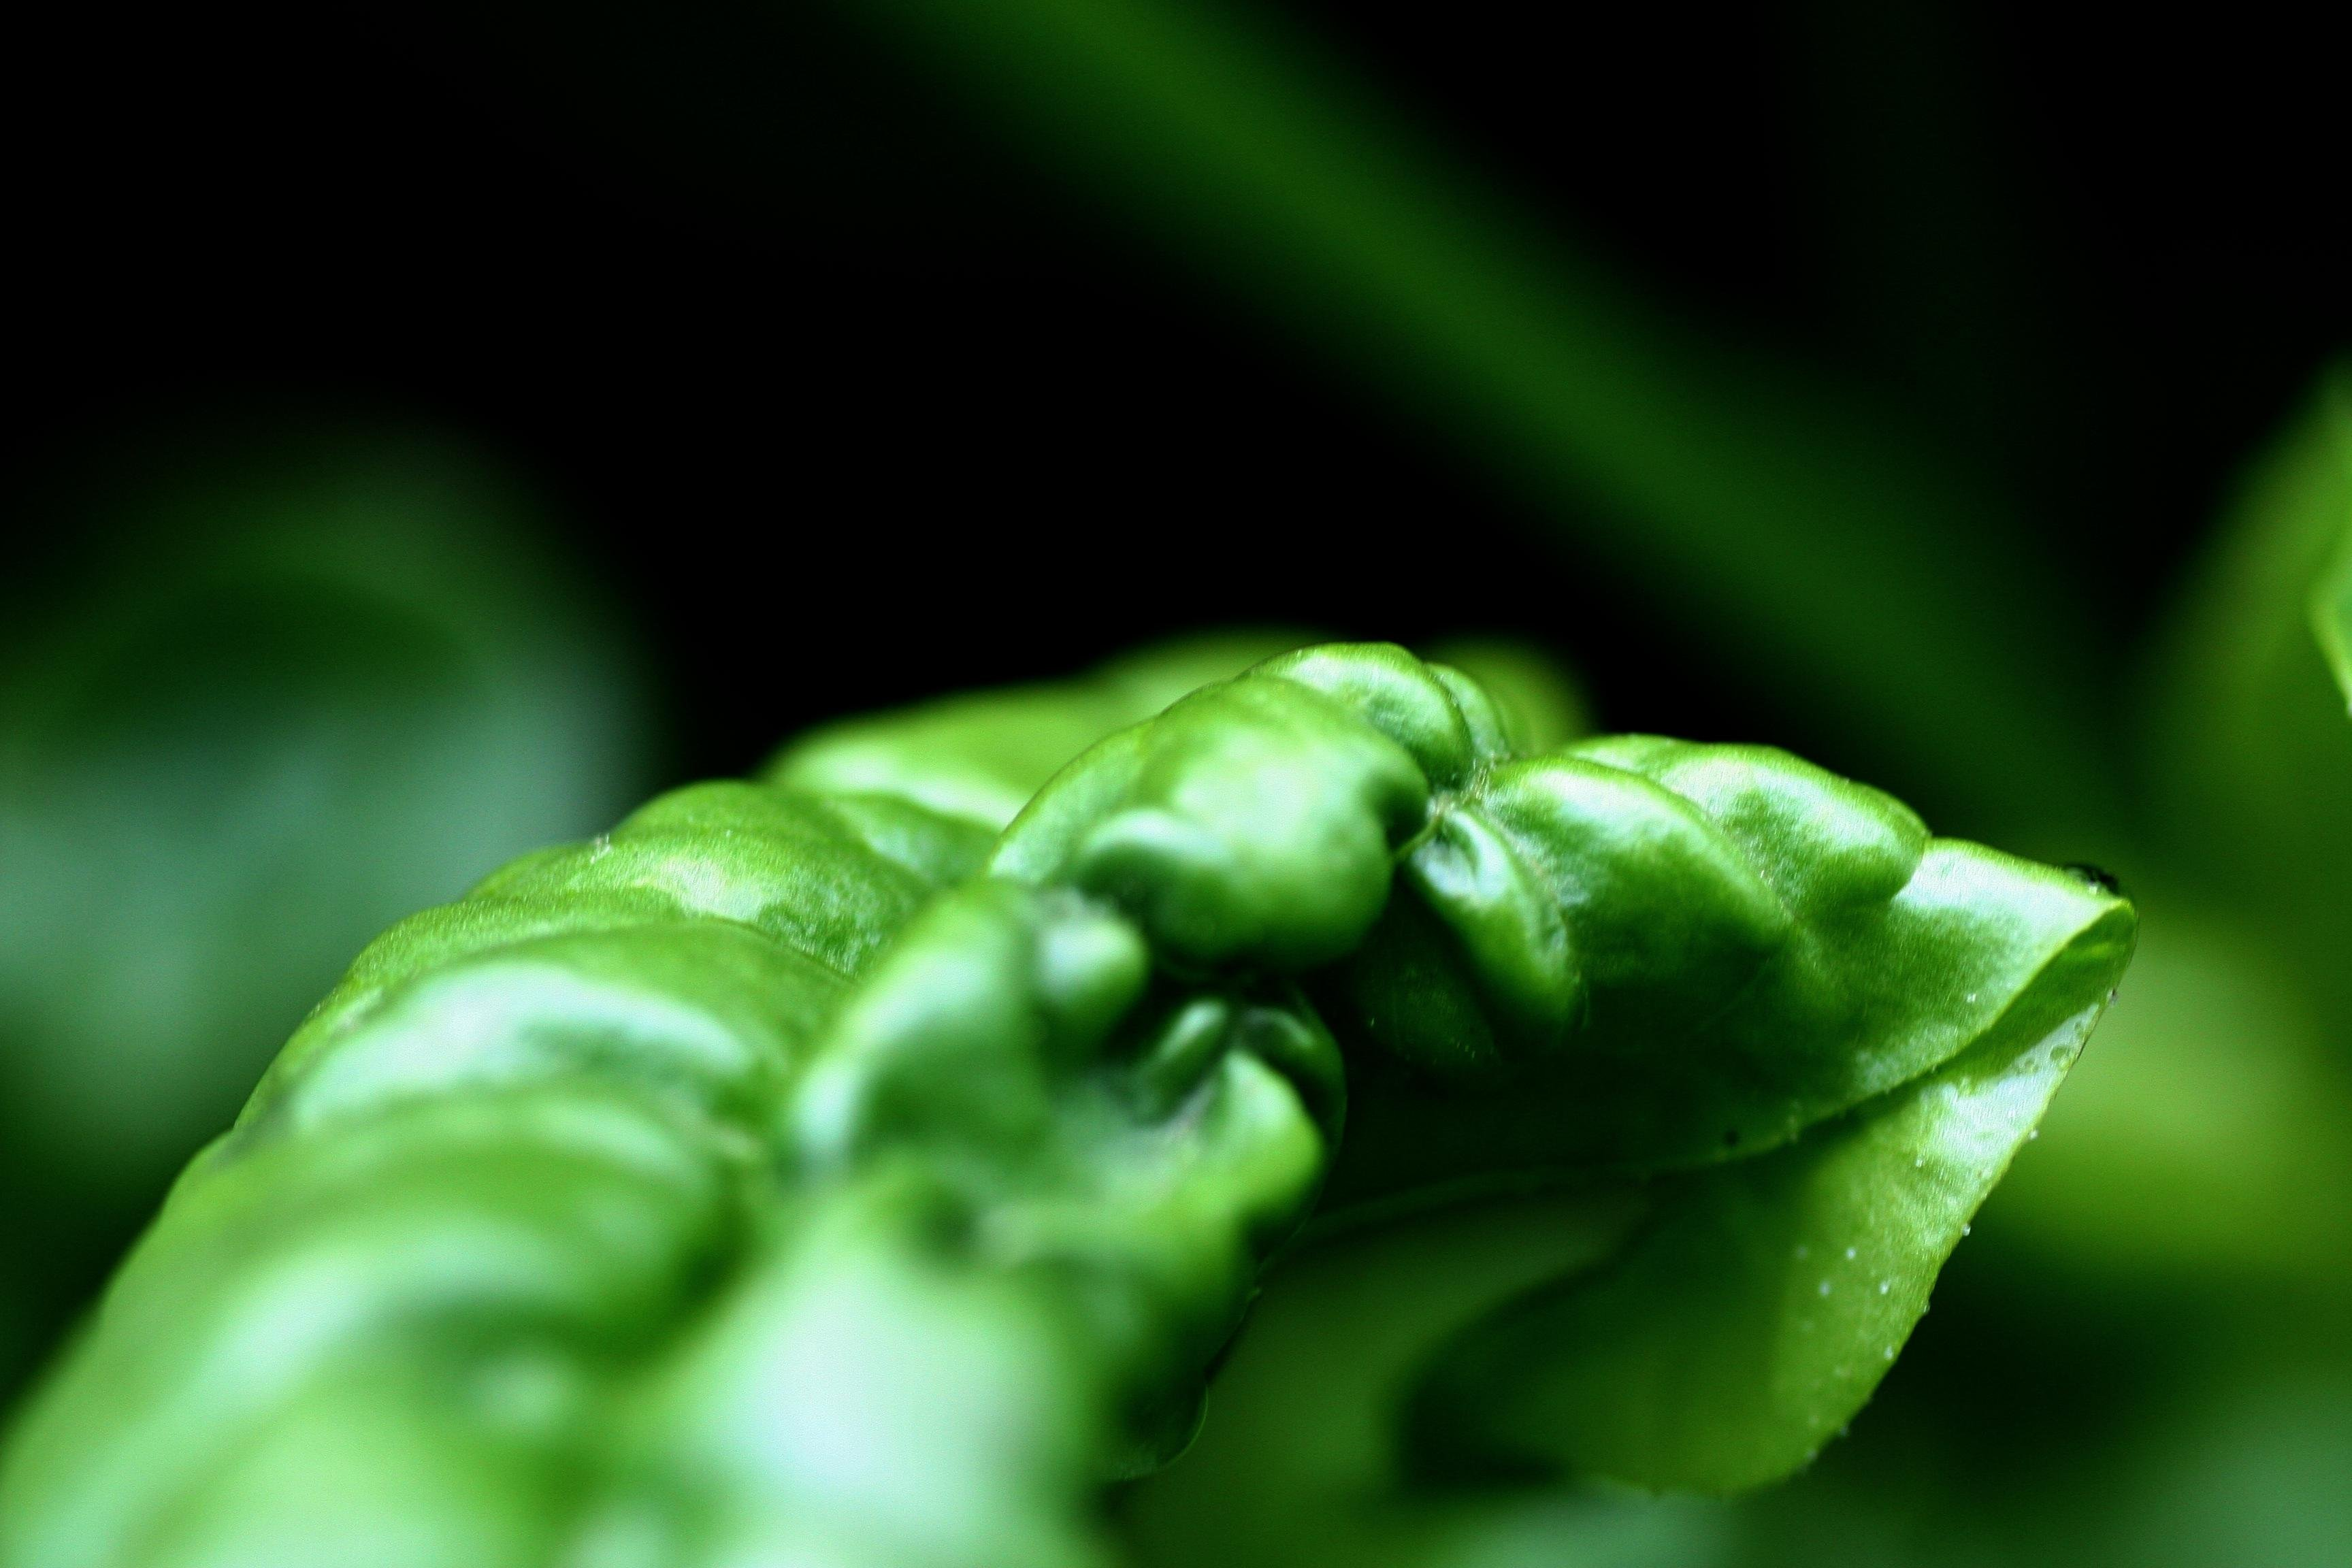
\includegraphics[width=\paperwidth,height=\paperheight]{spinach.jpg}
    \caption{Fresh Spinach}
\end{figure}
\restoregeometry
\clearpage

\section{Anne's Spinach Salad}
\begin{multicols*}{3}

\begin{quote}
    This recipe is from my Aunt Anne, who swears that she always used romaine lettuce instead of spinach.
\end{quote}

\begin{tabular}{r@{ }l}
    2 & eggs \\
\end{tabular}

Boil eggs, cool, shell and slice into rings.

\begin{tabular}{r@{ }l}
    10 & strips bacon \\
\end{tabular}

Separate strips onto aluminum foil in a baking sheet, and bake for 15 minutes at 425. Pat dry and chop into small pieces.

\begin{tabular}{r@{ }l}
    \sfrac{1}{2} & cup olive oil \\
    \sfrac{3}{4} & can anchovies in oil \\
               2 & tablespoons balsamic \\
               2 & tablespoons lemon juice \\
               1 & garlic clove \\
    \sfrac{1}{2} & teaspoon thyme \\
    \sfrac{1}{4} & teaspoon \\
                 & sugar \\
                 & oregano \\
                 & mustard powder \\
                 & onion salt \\
                 & paprika \\
\end{tabular}

Discard the oil in the can and use only the anchovies. Liquefy all  ingredients in a blender.

\begin{tabular}{r@{ }l}
    1 & package spinach \\
      & pre-sliced mushrooms \\
\end{tabular}

Combine eggs, bacon and dressing in a large mixing bowl.

\begin{quote}
The dressing can keep at least overnight.

To shell eggs easily, run under cold water, shaking pan to smash shells. The water will seep in. In 10 minutes, the shells will come off easily.

Leftover spinach can be saved, but be sure to reseal it in the original packaging, which is specially designed to breath. Spinach or lettuce saved in regular plastic will rot in a few days.

If you want to chop bacon very fine, freeze it for 10 minutes first.
\end{quote}

\end{multicols*}

\clearpage


\fullpageimage{couscous.jpg}{http://www.flickr.com/photos/stone-soup}

\section{Couscous Salad}
\begin{recipe}

\pre{
    Couscous has a tendency to clump together. Ideally, we want every kernel to be separate. Also, you want to serve the final salad as cold as possible. That means no lukewarm couscous.
}

\ingredients{
    1 & handful kosher salt \\
    3 & trays ice cubes \\
}

In one large metal bowl, combine ice, kosher salt, and enough water to cover the ice fully.

\ingredients{
    2 & boxes plain couscous \\
    1 & tablespoon butter \\
}

Follow the directions on the box to hydrate couscous. Immediately after the couscous is cooked, turn out into another metal bowl.

\columnbreak

\ingredients{
    \sfrac{1}{2} & cup Italian dressing \\
}

Mix the dressing into the couscous to help it separate. Fluff with a spatula, breaking up as many clumps as possible.

Place the metal bowl with the couscous into the bowl with the ice. Keep stirring every three minutes to break down the clumps.

\ingredients{
                6 & ounces feta cheese \\
                1 & orange bell pepper \\
                1 & yellow bell pepper \\
     \sfrac{1}{2} & large red onion \\
}

Dice the peppers and onion fine, and combine with feta cheese in the couscous bowl.

\ingredientsLeft{
    & Italian dressing \\
    & kosher salt \\
    & pepper \\
    & dried dill \\
}

Season to taste.

\columnbreak

\tip{
    The two large metal bowls with ice water is great for cooling just about anything quickly. It's kind of like a reverse double-boiler.
}

\tip{
    The boxed Couscous sold in the grocery store is actually pre-cooked, which is why it only takes a few minutes to hydrate. You can buy uncooked Couscous, which has larger grains and cooks like pasta.
}

\tip{
    When buying feta, I prefer the cryo-packed version with a little bit of juice sealed in. The free-standing feta in juice and the Saran-wrapped versions are dryer.
}

\end{recipe}

\section{Potato Salad}
\begin{recipe}

\pre{
    The key to this potato salad is cooking and cooling the potatoes completely, before 
    cutting them up, or stirring them. Otherwise, the potatoes start to break down and 
    muddy the salad. While they are hot, you want to both salt and season them with 
    vinegar (pickle juice). If you can cook the potatoes inside a fitted colander inside 
    a large pot, then they will bairly be distrubuted while cooking or cooling. 
}

\ingredients{
    3 & pounds medium or small yukon gold potatoes \\
    4 & quarts water \\
    & kosher salt \\    
    & pickle juice \\ 
}

Heavily salt water, put potatoes in, and bring to a boil. The water does not need to 
be at a boil before you put the potatoes in. Once boiling, reduce heat to a 
medium boil. Cook for 15 to 25 minutes, or until a knife easily pierces a potato. 

Drain potatoes using a colander. Place a colander with potatoes inside a large bowl. 
Pour (strained) pickle juice over the hot potatoes. Using another large bowl, move 
colander back and forth, and continue to pour the pickle juice over the potatoes every 
minute, until they stop steaming.

Leave potatoes out at room temperature to cool completely, before cutting them. 

\ingredients{
                2 & cups mayonnaise \\
                3 & celery stalks \\
                1 & small white onion \\
                1 & tablespoon celery seed \\
                2 & tablespoons dijon mustard \\
                3 & sprigs fresh dill \\
                  & fresh parsley \\
}

Dice celery, onion, dill and parsley fine. Whisk to combine with wet ingredients.
Season to taste with salt and pepper.

\ingredients{
      & paprika \\
}

Combine the potatoes and sauce, and top with paprika.

\end{recipe}


\listoffigures

\end{document}
